\documentclass[11pt]{report}

%-------------------------------------------------------------------------------------------------%

% PAQUETES

\usepackage[a4paper, right = 0.8in, left = 0.8in, top = 0.8in, bottom = 0.8in]{geometry}
\usepackage[utf8]{inputenc}
\usepackage[spanish]{babel}
\usepackage{amsmath,amsfonts,amssymb,amsthm}
\usepackage{multicol}
\usepackage{fouriernc}
\usepackage{enumitem}
\usepackage{mathtools} % Solo uso \underbracket
\usepackage{cellspace, tabularx, booktabs} % Líneas del título
\usepackage{parskip}
\usepackage{pdfpages}
\usepackage{cancel}

%-------------------------------------------------------------------------------------------------%

% AJUSTES GENERALES

\setlist[enumerate]{label={\textit{\alph*})}}

\makeatletter % Para quitar el espacio adicional que el paquete parskip añade al principio y al final de una demostración
\renewenvironment{proof}[1][\proofname]{\par
  \pushQED{\qed}%
  \normalfont \topsep\z@skip % <---- changed here
  \trivlist
  \item[\hskip\labelsep
        \itshape
    #1\@addpunct{.}]\ignorespaces
}{%
  \popQED\endtrivlist\@endpefalse
}
\makeatother

%-------------------------------------------------------------------------------------------------%

% COMANDOS PERSONALIZADOS

\newcommand{\N}{\mathbb N}
\newcommand{\Z}{\mathbb Z}
\newcommand{\Q}{\mathbb Q}
\newcommand{\R}{\mathbb R}
\newcommand{\C}{\mathbb C}

\newcommand{\pars}[1]{\left( #1 \right)} % Paréntesis de tamaño automático
\newcommand{\comment}[1]{}

%-------------------------------------------------------------------------------------------------%

% EJERCICIOS Y SOLUCIONES

\newtheorem{ejercicio}{Ejercicio}
\addto\captionsspanish{\renewcommand*{\proofname}{Solución}}

%-------------------------------------------------------------------------------------------------%

\begin{document}

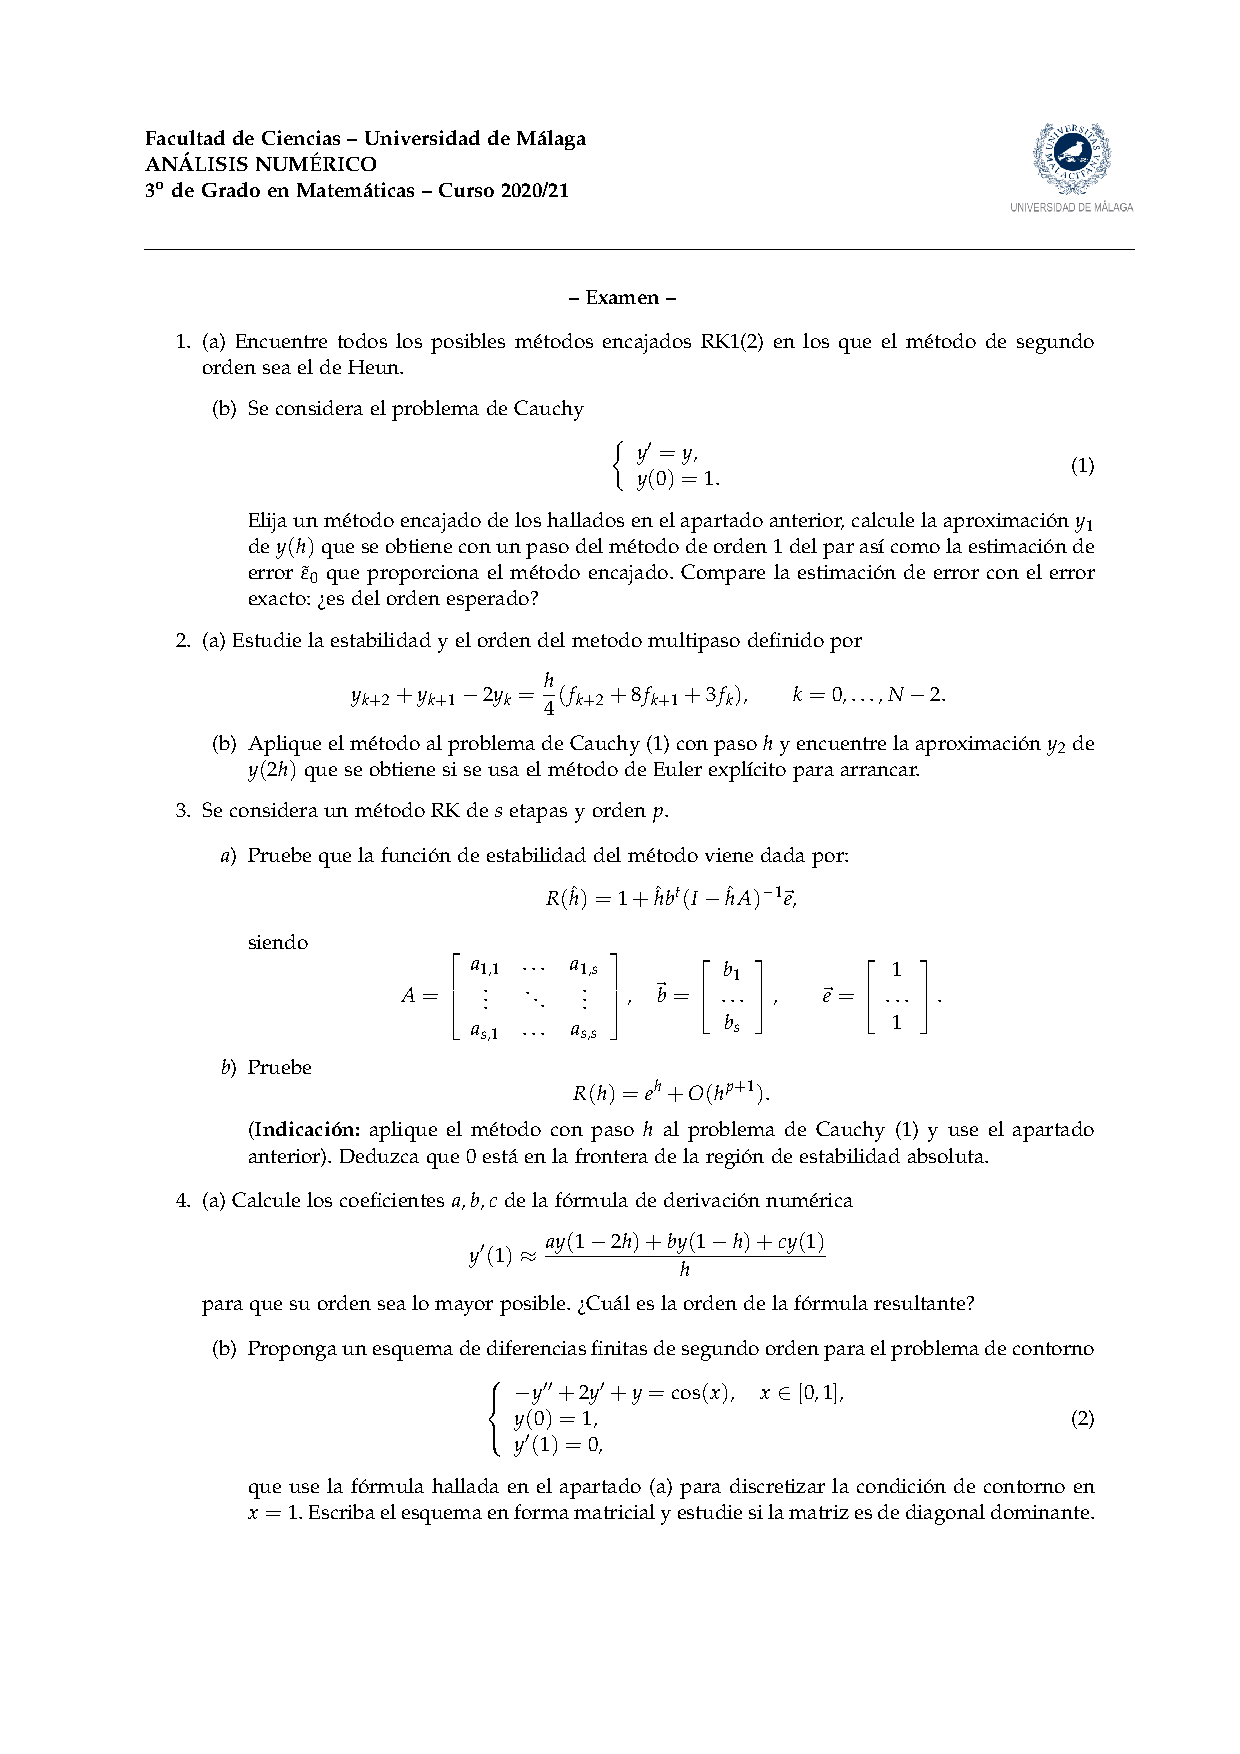
\includepdf[pages=-]{an_examen_2021-06.pdf}

%-------------------------------------------------------------------------------------------------%

% TÍTULO

\begin{center}

	\textbf{$-$ Resolución $-$}

\end{center}

%-------------------------------------------------------------------------------------------------%

\textbf{1.} No cae (menos mal).

\textbf{2. } 

\begin{enumerate}
    \item El mismo proceso de siempre:
    \[\sum_{j=0}^2 \alpha_j = 0, \qquad \sum_{j=0}^2 \alpha_jj = 1+2 = 3, \qquad \sum_{j=0}^2 \beta_j = \frac{1+8+3}{4} = 3,\]
    y el método es de orden $1$;
    \[\sum_{j=0}^2 \alpha_jj^2 = 1+4 = 5, \qquad \qquad 2\sum_{j=0}^2\beta_jj = 2\frac{8+2}{4} = 5,\]
    y el método es de orden $2$;
    \[\sum_{j=0}^2 \alpha_jj^3 = 1+8 = 9, \qquad \qquad 3\sum_{j=0}^2 \beta_jj^2 = 3\frac{8+4}{4} = \frac{36}{4} = 9,\]
    y el método es de orden $3$;
    \[\sum_{j=0}^2 \alpha_jj^4 = 1+16 = 17, \qquad \qquad 4\sum_{j=0}^2 \beta_jj^3 = 4 \frac{8+8}{4} = 16 \neq 17\]
    El método es de orden exactamente $3$.
    \item Al aplicar el método con $f(t,y)$ se obtiene
    \[y_{k+2}+y_{k+1}-2y_k = \frac{h}{4}(y_{k+2}+8y_{k+1}+3y_k) = \frac{h}{4}y_{k+2}+2hy_{k+1}+\frac{3h}{4}y_k,\]
    es decir,
    \[y_{k+2}= \frac{2hy_{k+1}+\frac{3h}{4}y_k-y_{k+1}+2y_k}{1-\frac{h}{4}} = \frac{(2h-1)y_{k+1}+(\frac{3h}{4}+2)y_k}{1-\frac{h}{4}}\]
    En particular, para $k = 0$,
    \[y(t_2) = y(2h) \approx y_{2}= \frac{(2h-1)y_{1}+(\frac{3h}{4}+2)y_0}{1-\frac{h}{4}}\]
    Hallemos $y_1$ mediante el método de Euler implícito, que aplicado a este problema es
    \[y_{k+1}=y_k+hy_{k+1},\]
    de donde
    \[y_{k+1} = \frac{y_k}{1-h}\]
    Por tanto,
    \[y_1 = \frac{y_0}{1-h} = \frac{1}{1-h}\]
    Volviendo arriba,
    \[y(2h) \approx y_{2}= \frac{(2h-1)\frac{1}{1-h}+\frac{3h}{4}+2}{1-\frac{h}{4}}\]
\end{enumerate}

\pagebreak

\textbf{3. }

\begin{enumerate}
    \item El método RK en cuestión viene dado por 
    \[\left\{\begin{alignedat}{1}
    y_k^{(1)} &= y_k+h(a_{1,1}f(t_k^{(1)},y_k^{(1)})+a_{1,2}f(t_k^{(2)},y_k^{(2)})+\mathellipsis+a_{1,s}f(t_k^{(s)},y_k^{(s)})) \\
    y_k^{(2)} &= y_k+h(a_{2,1}f(t_k^{(1)},y_k^{(1)})+a_{2,2}f(t_k^{(2)},y_k^{(2)})+\mathellipsis+a_{2,s}f(t_k^{(s)},y_k^{(s)})) \\
    &\phantom{\vdots} \vdots \\
    y_k^{(p)} &= y_k+h(a_{s,1}f(t_k^{(1)},y_k^{(1)})+a_{s,2}f(t_k^{(2)},y_k^{(2)})+\mathellipsis+a_{s,s}f(t_k^{(s)},y_k^{(s)})) \\
    y_{k+1} &= y_k+h(b_1f(t_k^{(1)},y_k^{(1)})+\mathellipsis+b_sf(t_k^{(s)},y_k^{(s)}))
    \end{alignedat}\right.\]
    Al aplicar el método al problema test de Dahlquist, es decir, poniendo $f(t,y)=\lambda y$, se obtiene, llamando $\hat{h}=\lambda h$,
    \[\left\{\begin{alignedat}{1}
        y_k^{(1)} &= y_k+\hat{h}(a_{1,1}y_k^{(1)}+a_{1,2}y_k^{(2)}+\mathellipsis+a_{1,s}y_k^{(s)}) \\
        y_k^{(2)} &= y_k+\hat{h}(a_{2,1}y_k^{(1)}+a_{2,2}y_k^{(2)}+\mathellipsis+a_{2,s}y_k^{(s)}) \\
        &\phantom{\vdots} \vdots \\
        y_k^{(p)} &= y_k+\hat{h}(a_{s,1}y_k^{(1)}+a_{s,2}y_k^{(2)}+\mathellipsis+a_{s,s}y_k^{(s)}) \\
        y_{k+1} &= y_k+\hat{h}(b_1y_k^{(1)}+\mathellipsis+b_sy_k^{(s)})
        \end{alignedat}\right.\]
    Sea 
\[Y = \left(\begin{array}{c}
    y_k^{(1)} \\
    y_k^{(2)} \\
    \vdots \\
    y_k^{(s)}
\end{array}\right)\]
Entonces el método se puede abreviar como
\[\left\{\begin{alignedat}{1}
    Y &= y_k\vec{e}+\hat{h}AY \\
    y_{k+1} &= y_k+\hat{h}b^tY
    \end{alignedat}\right.\]
De la primera ecuación se obtiene
\[(I-\hat{h}A)Y = y_k\vec{e}, \]
es decir,
\[Y = y_k(I-\hat{h}A)^{-1}\vec{e}\]
Sustituyendo en la segunda,
\[y_{k+1}=y_k+y_k\hat{h}b^t(I-\hat{h}A)^{-1}\vec{e} = (1+\hat{h}b^t(I-\hat{h}A)^{-1}\vec{e})y_k\]
Razonando por recurrencia,
\[y_k =(1+\hat{h}b^t(I-\hat{h}A)^{-1}\vec{e})y_{k-1} = (1+\hat{h}b^t(I-\hat{h}A)^{-1}\vec{e})^2y_{k-2} = \mathellipsis = (1+\hat{h}b^t(I-\hat{h}A)^{-1}\vec{e})^ky_0, \]
así que la función de estabilidad absoluta del método es
\[R(\hat{h}) = 1+\hat{h}b^t(I-\hat{h}A)^{-1}\vec{e}\]
\item Como el método es de orden $p$, entonces $\varepsilon_0 = O(h^{p+1})$. Pero
\[\varepsilon_0 = y(t_1)-y(t_0)-h\Phi(t_0,y_0,h) = y(t_1)-y_0-h\Phi(t_0,y_0,h) \tag{$\ast$}\]
En el problema $(1)$ se tiene que $y(t)=e^t$, $t_0 = 0$, $t_1 = h$ e $y_0 = 1$. Además, como se ha visto en el apartado anterior,
\[y_{k+1}=y_k+y_k\hat{h}b^t(I-\hat{h}A)^{-1}\vec{e}\]
Usando que en el problema $(1)$ es $\hat{h} = h$ (pues $\lambda = 1$),
\[y_{k+1}=y_k+hy_kb^t(I-\hat{h}A)^{-1}\vec{e},\]
deduciéndose que
\[\Phi(t_k,y_k,h) = y_kb^t(I-\hat{h}A)^{-1}\vec{e}\]
En consecuencia, llevando todo esto a $(\ast)$,
\[\varepsilon_0 = e^h-1-hb^t(I-\hat{h}A)^{-1}\vec{e} = e^h-R(h)\]
Esto nos dice que $e^h-R(h)=O(h^{p+1})$, o sea, $R(h)=e^h+O(h^{p+1})$.
\end{enumerate}

\textbf{4. } Lo mismo de siempre.

\end{document}